
% The \phantomsection command is needed to create a link to a place in the document that is not a
% figure, equation, table, section, subsection, chapter, etc.
% https://tex.stackexchange.com/questions/44088/when-do-i-need-to-invoke-phantomsection
\phantomsection

\chapter{Experiments}\label{chap:experiments}

To address the objective of this dissertation, experiments are conducted to evaluate learning-based primal heuristics for Mixed-Integer Linear Programming (MILP).
The ONTS problem (see Chap.~\ref{chap:onts}) serves as a realistic application to benchmark the selected techniques.

As discussed in Section~\ref{sec:onts-problem-statement}, during mission execution (with the nanosatellite in orbit), a new schedule must be generated during the communication window.
This involves optimizing multiple instances of the ONTS problem, given varying sets of tasks and updated nanosatellite information.
Each set of tasks is evaluated based on the resulting schedule, in an iterative process of including new tasks until scheduling becomes infeasible.
Therefore, during the communication window, quickly finding a good solution to a problem instance is more crucial than finding an optimal solution.
In other words, an efficient heuristic is crucial to allow for more iterations, which leads to a better set of tasks scheduled for execution.

The remaining of this chapter details the development and the experiments with the proposed learning-based heuristics for the ONTS problem.
This includes data acquisition, solution prediction model architecture, model training, and experiment setup.
Furthermore, the performance of the proposed learning-based heuristics is assessed on realistic instances of the ONTS problem.


\section{Data}

High-quality data is necessary both to train solution prediction models and to evaluate the proposed learning-based heuristics for the ONTS problem.
The datasets for both training and evaluation must be composed of instance-solution pairs, as discussed in Sec.~\ref{sec:training-solution-prediction}.
The quality of these instance-solution pairs is measured through their faithfulness, both the instance with respect to the true data distribution, and the solution with respect to the optimal.

\subsection{Instance space: the FloripaSat I mission}\label{sec:instance-space}

The instance space is defined from the parameters of the FloripaSat-I mission~\cite{marcelinoCriticalEmbeddedSystem2020}.
Their nanosatellite is in orbit at an altitude of 628 kilometers and an orbital period of 97.2 minutes.
The planning horizon is fixed at $T=125$ time slots, with one slot per minute, to account for a continuous scheduling, allowing for task executions that extend the communication window.
Any instance $I\in \mathcal{I}$ has either 9, 13, 18, 20, 22, or 24 tasks.

Once the orbit of the FloripaSat-I is stable and its received solar flux is constant, the power input vector $\bm{r}$ can be calculated deterministically from solar irradiance measurements as in \citeonline{morschfilhoComprehensiveAttitudeFormulation2020}.
2 years of solar irradiance data is used as a basis for the power input vectors of the instances in the instance space.
The set $R$ is used to denote all possible values of $\bm{r}$ from the historical data.
The other battery-related parameters (see Sec.~\ref{sec:onts-milp-formulation}) are fixed as 
\begin{align*}
    e &= 0.9 \\
    Q &= 5 \\
    \gamma &= 5 \\
    V_b &= 3.6 \\
    \rho &= 0.0
\end{align*}

The remaining parameters are constrained to ranges that match previous works in the area~\cite{rigoBranchandpriceAlgorithmNanosatellite2022,semanEnergyAwareTaskScheduling2022,rigoTaskSchedulingOptimal2021}.
Therefore, following the notation established in Sec.~\ref{sec:onts-milp-formulation}, the parameter space is defined as \[
\Pi = \bigcup_{\substack{J \in \left\{ 9,13,18,20,22,24 \right\} \\ T \in \left\{ 125 \right\} }} \Pi^{J,T}
,\] where each $\Pi^{J,T}$ is such that a parameter vector \[
\pi_I= \left( \bm{u}, \bm{q}, \bm{y}^{\min}, \bm{y}^{\max}, \bm{t}^{\min}, \bm{t}^{\max}, \bm{p}^{\min}, \bm{p}^{\max}, \bm{w}^{\min}, \bm{w}^{\max}, \bm{r}, \rho, e, Q, \gamma, V_b \right)
\] belongs to $\Pi^{J,T}$ if, and only if,
\begin{equation*}
\begin{aligned}
&\begin{rcases}
    & u_j \in [1, J] \\
	 & q_j \in [0.3, 2.5] \\
    	 & y_j^{\min} \in [1, \lceil T/45 \rceil] \\
    	 & y_j^{\max} \in [y_j^{\min}, \lceil T/15 \rceil] \\
    	 & t_j^{\min} \in [1, \lceil T/10 \rceil] \\
    	 & t_j^{\max} \in [t_j^{\min}, \lceil T/4 \rceil] \\
    	 & p_j^{\min} \in [t_j^{\min}, \lceil T/4 \rceil] \\
    	 & p_j^{\max} \in [p_j^{\min}, T] \\
    	 & w_j^{\min} \in [0, \lceil T/5 \rceil] \\
    	 & w_j^{\max} \in [\lfloor T-\lceil T/5 \rceil \rfloor, T]
\end{rcases} \forall j =1,\ldots,J \\
    &\quad \bm{r} \in R \\
    &\quad e = 0.9 \\
    &\quad Q = 5 \\
    &\quad \gamma = 5 \\
    &\quad V_b = 3.6 \\
    &\quad \rho = 0.0
.\end{aligned}
\end{equation*}
Finally, the input space is then define from the parameter space, such that \[
    I\in \mathcal{I} \iff \pi_I \in \Pi 
.\] 


\subsection{Data acquisition}\label{sec:data-acquisition}

As historical data is not available for the ONTS problem, the dataset is built from randomly generated instances sampled uniformly from the instance space of the FloripaSat-I mission.
More precisely, the dataset is built with instances drawn uniformly from the instance space defined above.

As the addition of an element to the dataset requires a solution to the ONTS problem, the computational cost of building a large dataset with hard instances is very high.
To alleviate this cost, the training set is built solely with instances with fewer tasks, which are, on average, faster to solve than instances with many tasks.
However, the instances of interest are those with plenty of tasks, which are harder to solve in practice, and, thus, motivate the use of heuristics.
Therefore, the validation and test datasets are built from instances with many tasks, which are, on average, significantly harder to solve.
Table~\ref{tab:dataset} details the number of instances by size (number of tasks) in each dataset generated.

\begin{table}[h]
    \centering
    \caption{Number of instances by size in each dataset. The datasets were generated through Algorithm~\ref{alg:dataset-generation}.}
    \label{tab:dataset}
    \begin{tabular}{l | c | c | c}
    \toprule
    & Training & Validation & Test \\
    \midrule
    $J = 9$ & 200 & 0 & 0 \\
    $J = 13$ & 200 & 0 & 0 \\
    $J = 18$ & 200 & 0 & 0 \\
    $J = 20$ & 0 & 20 & 20 \\
    $J = 22$ & 0 & 20 & 20 \\
    $J = 24$ & 0 & 20 & 20 \\
    \midrule
    Total & 600 & 60 & 60 \\
    \bottomrule
    \end{tabular}
\end{table}

Distinguishing the size of the instances in each dataset allows for the construction of a large training set, which enables the models to properly learn the problem, while maintaining a challenging evaluation scenario.
On top of that, this approach also enables the evaluation of the generalization capabilities of the proposed solution prediction models and the derived learning-based heuristics.

The algorithm to generate the datasets is presented in Algorithm~\ref{alg:dataset-generation}.
As the time horizon is fixed, the algorithm is executed once for each number of tasks possible.
Every new instance $I$ is solved using the SCIP solver~\cite{bestuzhevaSCIPOptimizationSuite2021} with a limited time budget of 5 minutes.
An instance is rejected if no feasible solution is found during the time budget or if the solver proves infeasibility.
For each instance $I$ in the resulting dataset, the set $Z^*_I$ contains the best 500 solutions found by the solver.

\begin{algorithm}[h]
    \NoCaptionOfAlgo
    \SetAlgoLined
    \KwData{Time horizon $T$, number of jobs $J$, number of instances (final dataset size) $n$.}
    \KwResult{Dataset $\mathcal{D} = \{(I,Z_I^\star): Z_I^\star\subset Z_I\}$.}
    
    \While{$|\mathcal{D}| < n$}{
        $\pi \sim \mathcal{U}\left( \Pi^{J,T} \right) $ \\
        $I \gets {\tt ONTS}(\pi)$ \\
        $Z_I^\star \gets {\tt Solver}(I)$
        
        \If{$|Z_I^\star| > 0$}{%
            $\mathcal{D}$.add$(I, Z_I^\star)$
        }
    }
    \caption{\textbf{Algorithm 1:} Dataset generation algorithm. $\pi$ is the parameter vector and $\Pi^{J,T}$ is the parameter space (see Sec. \ref{sec:onts-milp-formulation}), $Z_I$ represents the set of all feasible solutions of instance $I$, and $Z_I^\star \subset Z_I$ the set of feasible solutions the solver finds.
    ${\tt ONTS}$ represents a function that takes as input a parameter vector and constructs an instance of the ONTS problem.
    ${\tt Solver}$ is any MILP solver.
    Note that the parameters are drawn uniformly from the parameter space.
    }\label{alg:dataset-generation}
\end{algorithm}


\section{Solution Prediction Model}

The instance space of the ONTS problem, as defined in Sec.~\ref{sec:instance-space}, imposes specific architectural requirements for solution prediction models.
The variable number of tasks over the instances of interest leads to parameter vectors of variable length, which is a natural embedding (feature vector) for the instances.
At the same time, the uneven number of tasks in the instance space implies that instances have different number of binary variables.
Therefore, models must predict a different number of variable assignments for each instance.

Graph Neural Networks (GNNs) are particularly promising in this context and are considered state-of-the-art for such applications~\cite{cappartCombinatorialOptimizationReasoning2022}.
As discussed in Sec.~\ref{sec:gnns}, GNNs naturally handle variable input and output sizes due to their convolutional nature.
On top of that, results shown by \citeonline{gasseExactCombinatorialOptimization2019} point that GNNs are capable of generalizing to instances larger than those seen during training, which alleviates data acquisition costs, as discussed in Sec.~\ref{sec:data-acquisition}.
Therefore, the deep learning models trained for the ONTS problem are all built with GNNs at their core.

\subsection{Instance embedding}

Because GNNs are at the core of the solution prediction models, the instances are embedded as bipartite graphs, following the approach presented in~\ref{sec:graph-embedding}.
Many authors have presented different approaches for defining node features when applying GNNs to MILP problems.
\citeonline{khalilMIPGNNDataDrivenFramework2022} add variable and constraint degrees\footnote{A variable's degree is the number of constraints in which it has a nonzero coefficient. On the other hand, a constraint's degree is the number of variables in it with non-zero coefficient.} to the baseline (the one presented in Sec.~\ref{sec:graph-embedding}) embedding.
\citeonline{chenRepresentingMixedIntegerLinear2022} embeds variables' upper and lower bounds as well as constraint set (inequality or equality).
Works that applied GNNs to generate branch-and-bound heuristics (e.g., for branching), such as \citeonline{dingAcceleratingPrimalSolution2020} and \citeonline{gasseExactCombinatorialOptimization2019}, have captured features usually available at the nodes of the branch-and-bound tree, directly collecting solver-computed features.
As the focus of the present work is on primal heuristics, the features should be solver-independent, i.e., they must be computed prior to the branch-and-bound application.

The resulting features used are based on the set proposed by \citeonline{hanGNNGuidedPredictandSearchFramework2023}, which extends both \citeonline{khalilMIPGNNDataDrivenFramework2022} and \citeonline{chenRepresentingMixedIntegerLinear2022} with simple features (solver-independent) that are also present in \citeonline{gasseExactCombinatorialOptimization2019}.
A summary is presented in Table~\ref{tab:feature-desc}.
Note that, following the literature, instead of describing all constraints as inequality constraints (i.e., in the normal form), the constraint type (inequality or equality) is informed through the constraint node features, reducing the graph size.
Furthermore, this feature design is problem agnostic, i.e., it does not use any information particular to the ONTS problem.

\begin{table}[h]
    \centering
    \begin{tabular}{p{7cm}|p{7cm}}
    \toprule
        Features of constraint nodes ($\bm{f}_{v_{\rm con}}$) & Features of variable nodes ($\bm{f}_{v_{\rm var}}$) \\
    \midrule
	Constraint's upper bound ($\bm{b}$)                     &  Variable's coefficient in the objective ($\bm{c}$)\\[0.8cm]
         Constraint's average coefficient (mean of $A_{i*}$)     &  Variable's average coefficient in the constraints (mean of $A_{*j}$) \\[0.8cm]
         Number of neighbors/non-null coefficients ($|\mathcal{N}(v_{\rm con})|$)    &  Number of neighbors/non-null coefficients ($|\mathcal{N}(v_{\rm var})|$) \\[0.8cm]
         Whether it is an equality or an inequality constraint &  Largest coefficient in the constraints ($\max(A_{*j})$) \\[0.8cm]
                                                                    &  Smallest coefficient in the constraints ($\min(A_{*j})$) \\[0.8cm]
                                                                    &  Whether it is a continuous or binary variable \\
    \bottomrule
    \end{tabular}
    \caption{Description of node features for the graph embedding of instances of the ONTS problem.}
    \label{tab:feature-desc}
\end{table}

\subsection{Architecture}

An architectural overview of the solution prediction models is illustrated in Fig.~\ref{fig:satgnn}.
The model inputs are the embedding described in the previous section, i.e., the bipartite graph representation of the instance and sets of feature vectors $F_\textrm{con}$ and $F_\textrm{var}$.

- illustration
- recall notation from 2.2.2
- the feature vectors are first encoded into a common hidden feature space using FCNs
- each layer of our model contains two passes, exploiting the bipartite nature of the input graph, following Gasse, which was also replicated by XXX
- finally, after L layers, the resulting hidden features are transformed in the predicted bias by another FCN

- describe hyperparameters that define the architecture

The architecture of the solution prediction model is illustrated in Figure \ref{fig:model-architecture}. As recalled from Sec.~2.2.2, the feature vectors are initially encoded into a common hidden feature space using Fully Connected Networks (FCNs). Each layer of our model comprises two passes that exploit the bipartite nature of the input graph, following the approach by Gasse et al., which was also replicated by subsequent studies.

%\begin{figure}[h]
%\centering
%\includegraphics[width=\textwidth]{model_architecture.png}
%\caption{Architecture of the solution prediction model.}
%\label{fig:model-architecture}
%\end{figure}

After \(L\) layers, the resulting hidden features are transformed into the predicted bias by another FCN. The model's hyperparameters, including the number of layers \(L\), the size of the hidden layers, and learning rates, are tuned to optimize performance on the ONTS problem.

\begin{figure}[h]
    \centering
    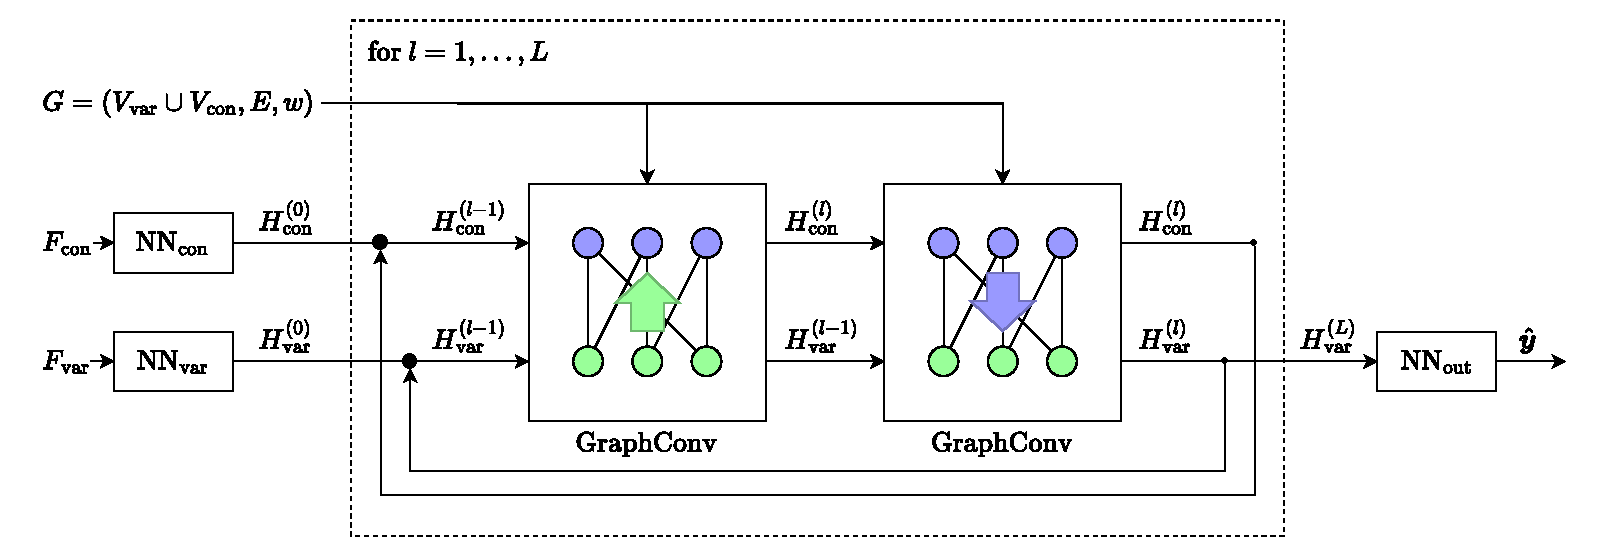
\includegraphics[width=\textwidth]{SatGNN.pdf}
    \caption{Architectural components of the solution prediction models trained for the ONTS problem.} % TODO: describe GraphConv, NNs sets F and H
    \label{fig:satgnn}
\end{figure}

% \begin{table}[h]
% \centering
% \begin{tabular}{|c|c|}
% \hline
% Hyperparameter & Value \\
% \hline
% Number of layers (L) & X \\
% Size of hidden layers & Y \\
% Learning rate & Z \\
% Batch size & W \\
% ... & ... \\
% \hline
% \end{tabular}
% \caption{Hyperparameters of the solution prediction model.}
% \label{tab:hyperparameters}
% \end{table}

\section{Training}

\section{Evaluation}

